%% part1
\MinParskip{}

\section{Basic Introduction}

\subsection{Background}
Light pollution is a term used to describe the excessive or inappropriate use of artificial light, which can take the form of light trespass, over-illumination, and light clutter. These phenomena are often visible as a glow in the night sky in large cities, but they can also occur in more remote areas. Light pollution affects our environment, health, and safety by altering our view of the night sky, delaying or accelerating plant maturation, disrupting wildlife migration patterns, and affecting our circadian rhythms. Excessive artificial light can lead to poor sleep quality and may contribute to physical and mental health problems, while glare from artificial lights can increase the risk of motor vehicle accidents.

\begin{figure}[H]\centering
    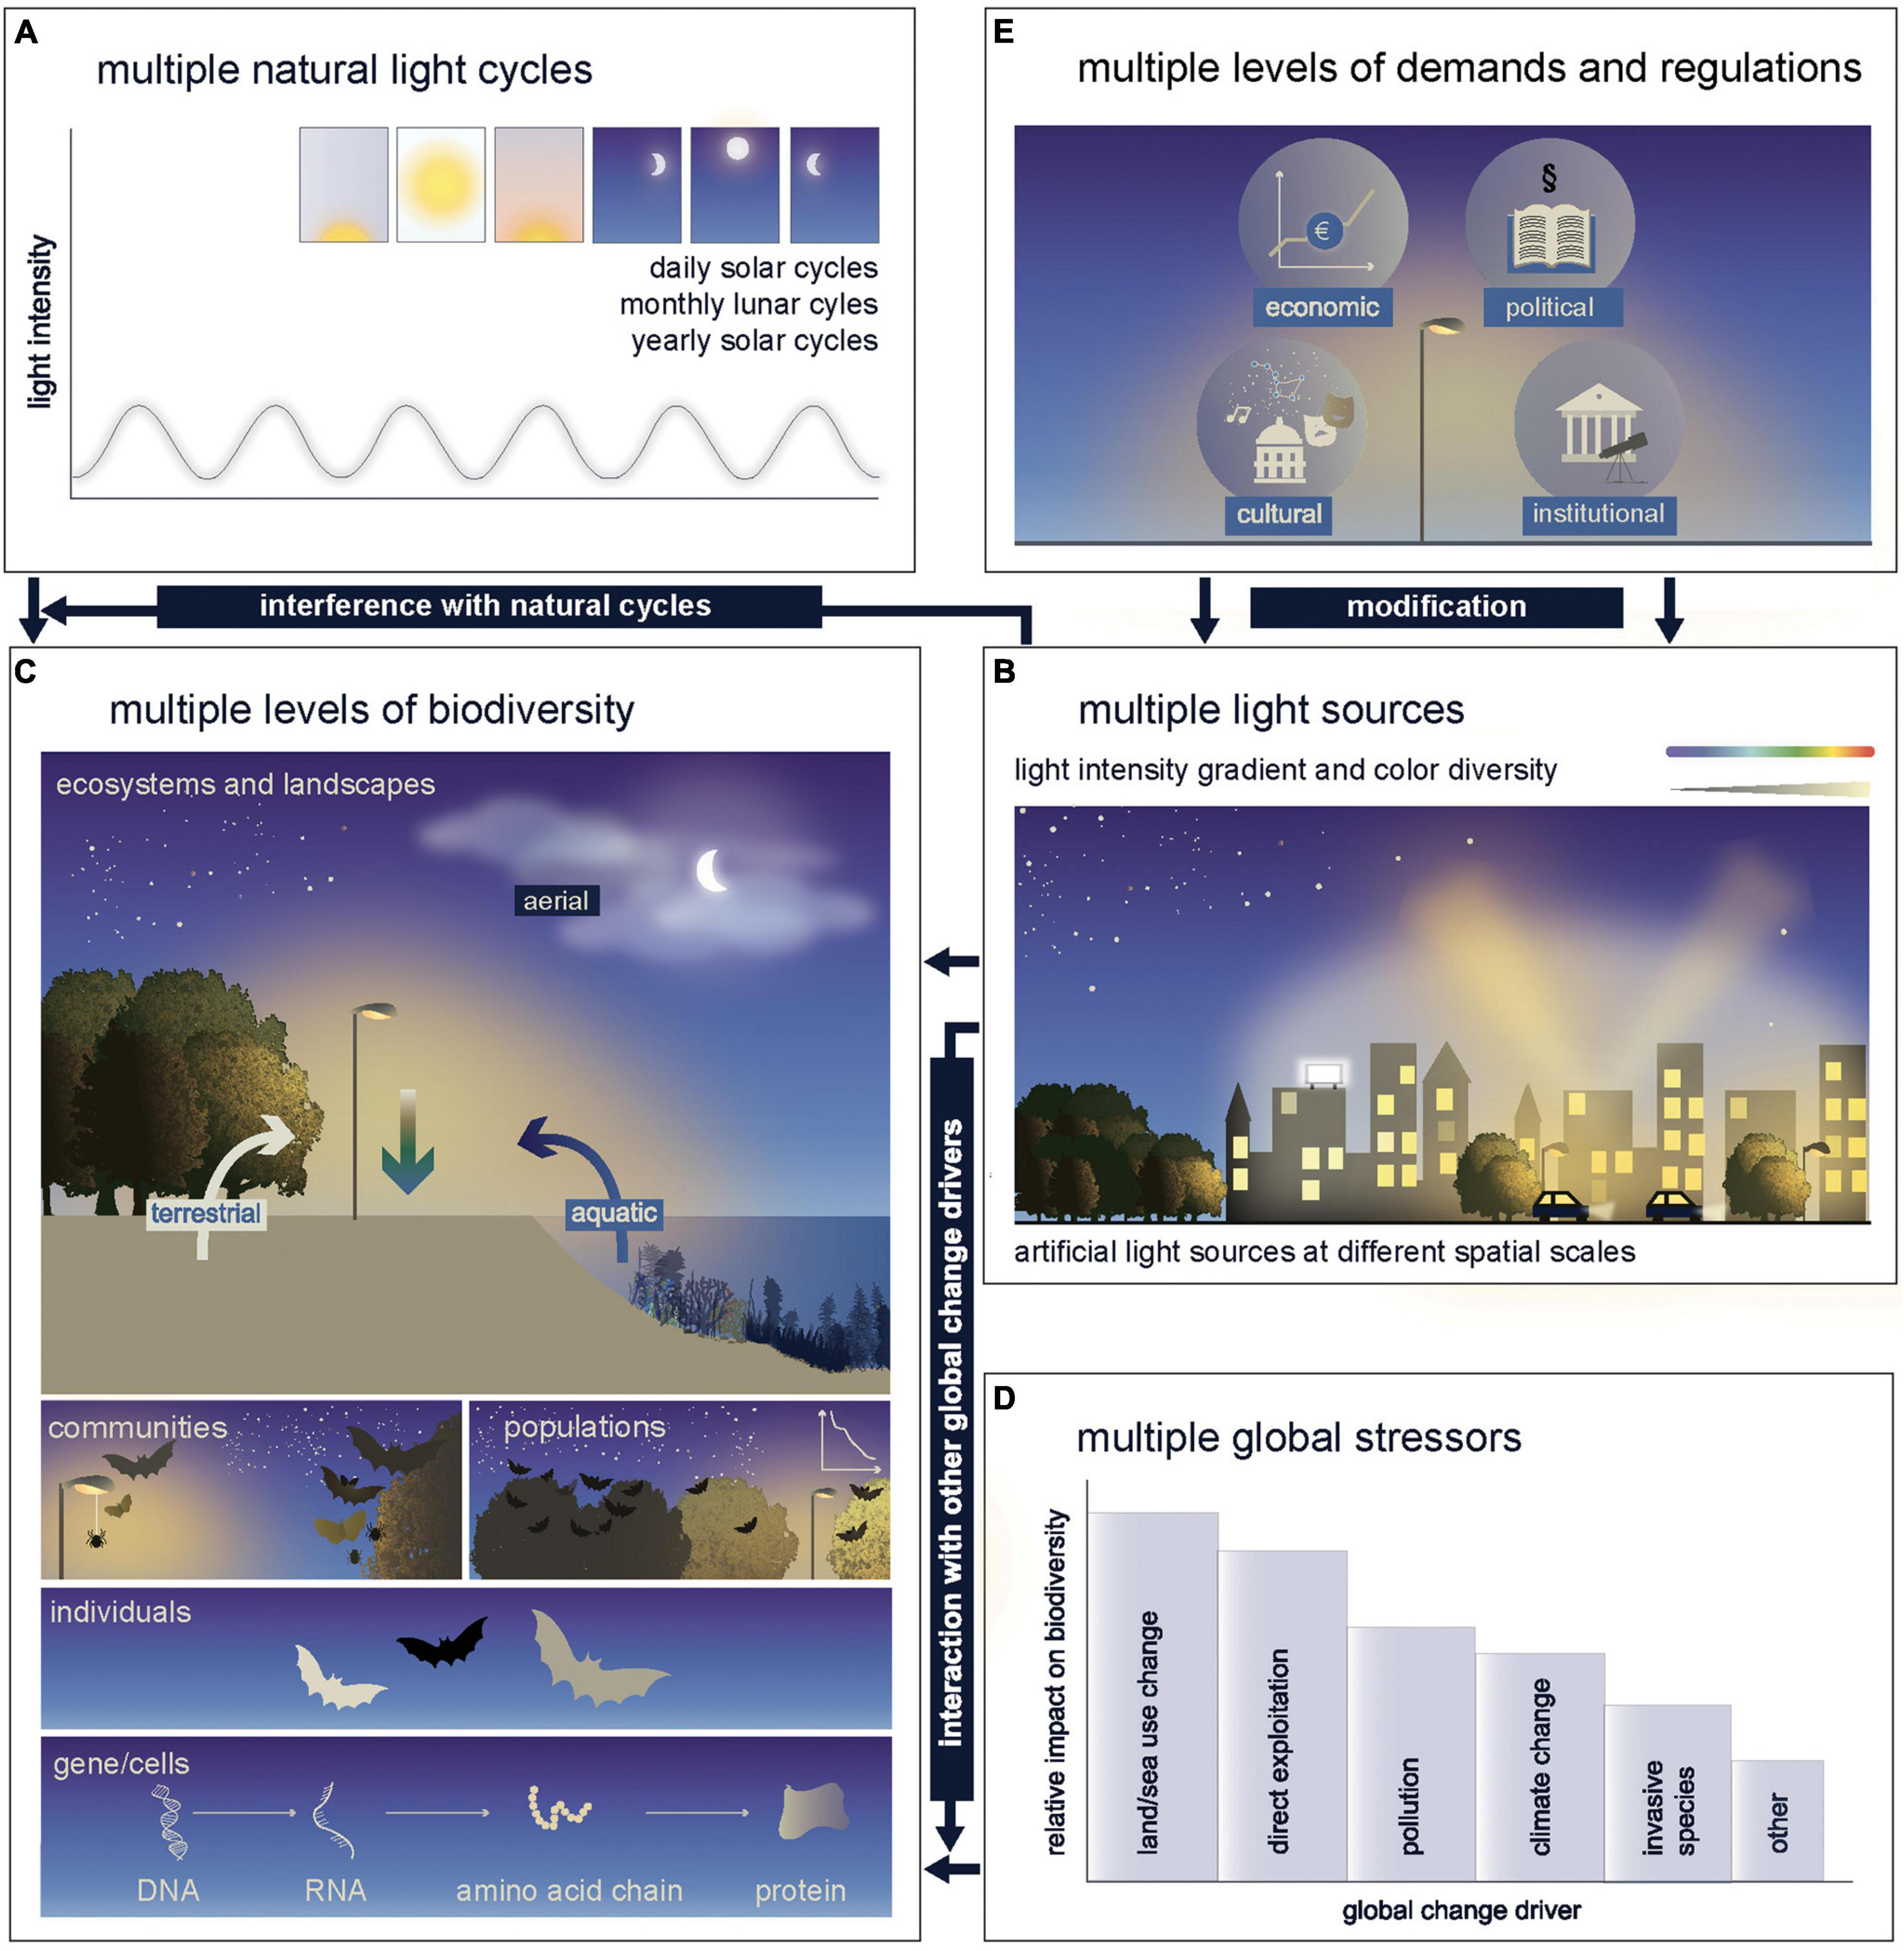
\includegraphics[width=0.9\textwidth]{figures/fevo-09-767177-g002.jpg}
    \caption{Artificial light at night: Potential sources, biodiversity impacts and responses are complex. Different natural light cycles (A) are affected by multiple forms of artificial light at night (B) at multiple levels of biodiversity in multiple realms (e.g. from bottom up: gene expression; phenotypes; population dynamics, e.g. decline; community composition; species dispersal and/or organismic fluxes across ecosystem boundaries and bioms) (C). Artificial light at night can interact with multiple global change stressors (D). Due to the potentially conflicting demands of artificial light at night a transition to a more sustainable use is extremely challenging and requires multiple levels of regulations (E) \cite{10.3389/fevo.2021.767177}} \label{fig:figure2}
\end{figure}

However, artificial light has both positive and negative impacts that can vary based on location. The effects of light pollution can depend on factors such as a location's level of development, population, biodiversity, geography, and climate. Therefore, assessing the extent of the effects and potential impacts of intervention strategies must be tailored to the specific location, and intervention strategies are needed to mitigate the negative effects of light pollution.

Light pollution is a serious problem with implications for wildlife, human health, scientific research, energy consumption, global warming, and the ageless pastime of observing the night sky. Pristinely dark skies are very scarce in the developed world and most of the world's population—and nearly all of those living in the EU or the US—live under skies with at least some light pollution\cite{GALLAWAY2010658}. 

For biodiversity studies, nocturnal light ideally would be measured in biologically relevant ways, based on thresholds and spectral sensitivities of the species, because different light sources interfere differently with the large diversity of sensory systems in nature\cite{davies2013artificial}.

\subsection{Problem Restatement}
\begin{itemize}
    \item The indicators of the EWM-TOPSIS model should be determined, in other words, it is equal to build a broadly applicable metric for identifying the light pollution risk level.
    \item Apply the indicators and the related data to the EWM-TOPSIS model, then analyse the result in the four diverse types of locations.
    \item Design 3 possible strategies for addressing light pollution, and how the indicators change with the strategies.
    \item Select 2 locations, and implement the most effective intervention strategies for each of them. See how the indicators change and the impact of the chosen intervention strategy.
    \item Write a 1-page flyer to community officials or local groups in a specific location to promote the most-effective intervention strategy tailored for the location.
\end{itemize}


\subsection{Our works}
First of all, we selected 9 cities as evaluation objects and 9 indicators for the EWM-TOPSIS Model. Both benefit-attributed and cost-attributed indicators are taken into account. Then we use the Entropy Weight Method (EWM) to get the weight of indicators. After getting the weights, we use the TOPSIS method to determine the best option from a set of alternatives.
\begin{figure}[H]\centering
    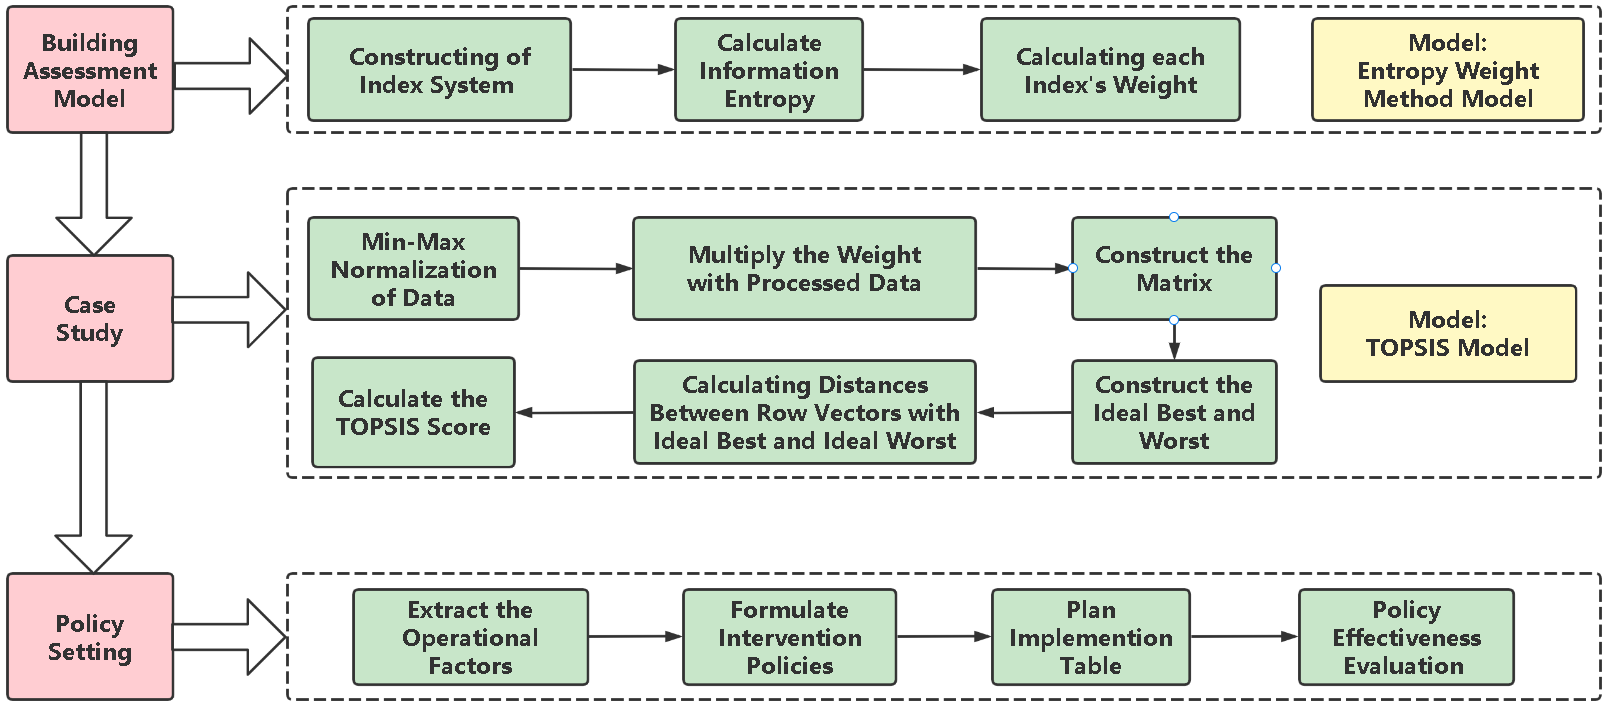
\includegraphics[width=1\textwidth]{figures/Flowchart}
    \caption{Our workflow.} \label{fig:figure1}
\end{figure}



